%________________________________________________________________________________________________
\documentclass{beamer}
%________________________________________________________________________________________________
\usepackage[french]{babel} 
\usepackage[utf8]{inputenc} 
\usepackage[T1]{fontenc} 
\usepackage{graphicx}
\usepackage[utf8]{inputenc}
\usepackage{fancyhdr}
\usepackage{geometry}
\usepackage{tabularx,tabulary}
\usepackage{movie15}
%________________________________________________________________________________________________
\title{3I013 Réunion du 29 Mars 2019}
\author{Daoud KADOCH\\Fabien MANSON\\Maël FRANCESCHETTI\\Nicolas CASTANET\\}
%________________________________________________________________________________________________
%ce theme est le plus clean de Beamer le truc a ne pas utiliser c'est 'Warsaw'
\usetheme{default}
%suppression de la barre de navigation inutile
\setbeamertemplate{navigation symbols}{}
\setbeamertemplate{frametitle}[default][center]

%\logo{
\includegraphics[height=0.5cm]{logo_sorbonne.png}}

%________________________________________________________________________________________________
\addtobeamertemplate{footline}{
	\begin{flushright}
	\vbox{\insertframenumber/\inserttotalframenumber}
	\end{flushright}}

%________________________________________________________________________________________________
\begin{document}


	%premiere diapo
	\begin{frame}
		\begin{center}
		\date{21 mars 2019}
		\maketitle
		\end{center}
	\end{frame}
	
	
	
	\begin{frame}
		\section{}
		\begin{flushleft}
		\frametitle{Sommaire}
		\tableofcontents{}
		\end{flushleft}
	\end{frame}
	
		\begin{frame}
	\section{Contexte}
		\begin{center}
		\frametitle{L'Objectif du Projet}
		%\subsection{Objectif}
        %\framesubtitle{L'expression des besoins}
		   Faire effectuer une ronde à un drone Bebop 2 en suivant un itinéraire prédéfini, tout en visualisant le retour vidéo en temps réel sur un iPod à travers un masque FPV.
		\end{center}
	\end{frame}
	
	\begin{frame}
	\section{Architecture Logicielle}
		\begin{center}
		\frametitle{Architecture Logicielle}
		%\subsection{Contraintes}
        %\framesubtitle{Les solutions}
       
        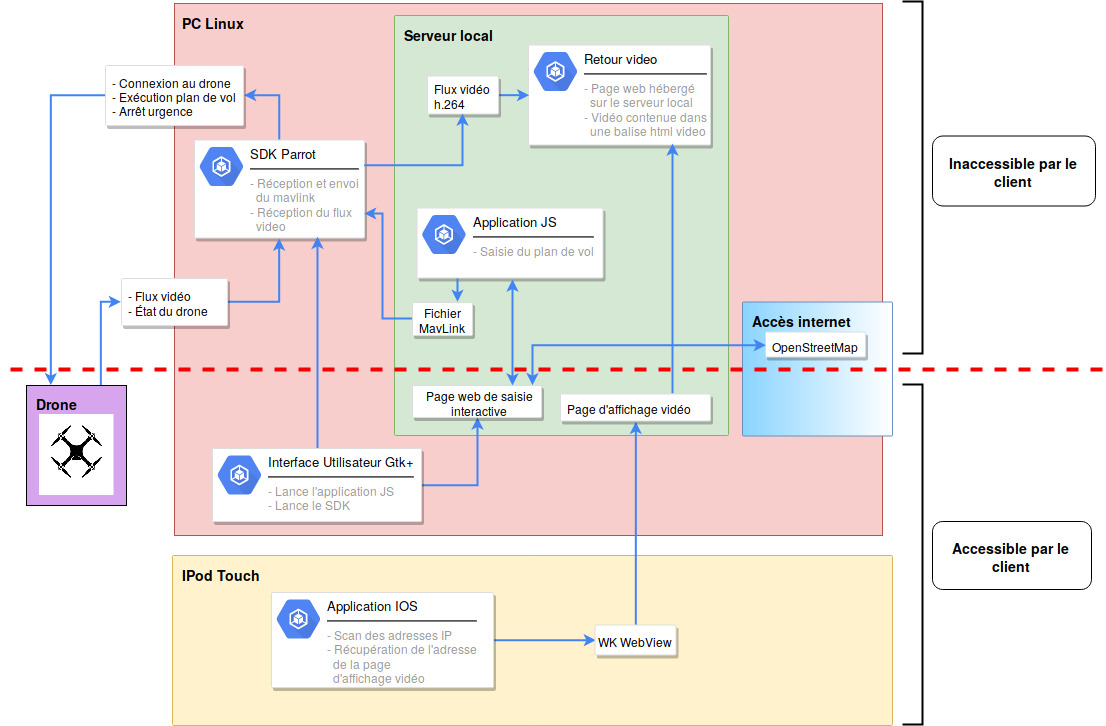
\includegraphics[scale=0.3]{Architecture_logicielle_v2.jpg}
		\end{center}
	\end{frame}
	
	\begin{frame}
	\section{SDK Parrot}
		\begin{center}
		\frametitle{SDK Parrot}
		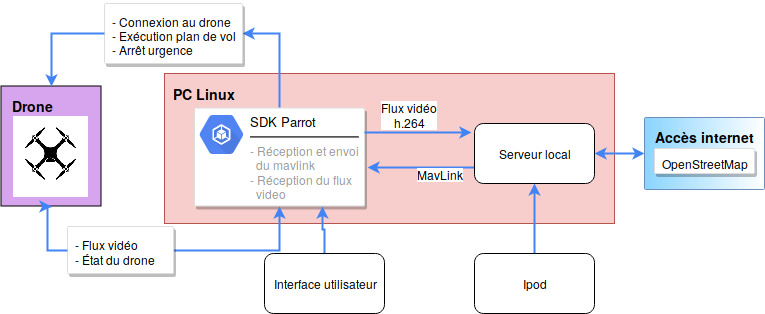
\includegraphics[scale=0.4]{SDK.jpg}
		\end{center}	
	\end{frame}
	
	\begin{frame}
	\section{Serveur local}
		\begin{center}
		\frametitle{Serveur local}
		%\subsection{Contraintes}
        %\framesubtitle{Les solutions}
        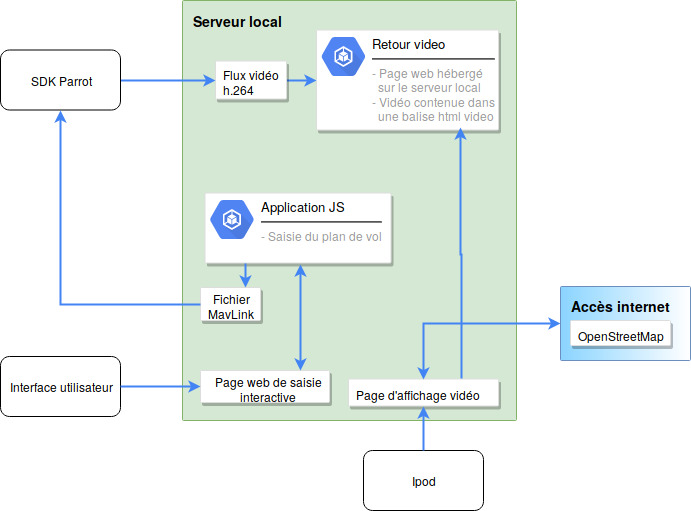
\includegraphics[scale=0.4]{Serveur.jpg}
		\end{center}
	\end{frame}
	
	
	\begin{frame}
	\section{App Ios}
		\begin{center}
		\frametitle{App Ios}
		%\subsection{Contraintes}
        %\framesubtitle{Les solutions}
        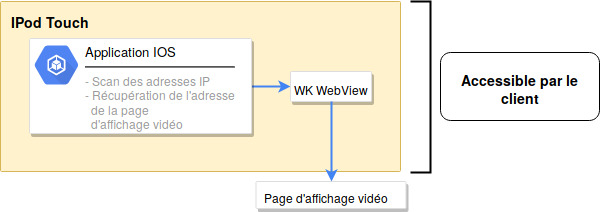
\includegraphics[scale=0.5]{ios_app.jpg}
		\end{center}
	\end{frame}
	
	\begin{frame}
	\section{App Ios}
		\begin{center}
		\frametitle{App Ios}
		%\subsection{Contraintes}
        %\framesubtitle{Les solutions}
        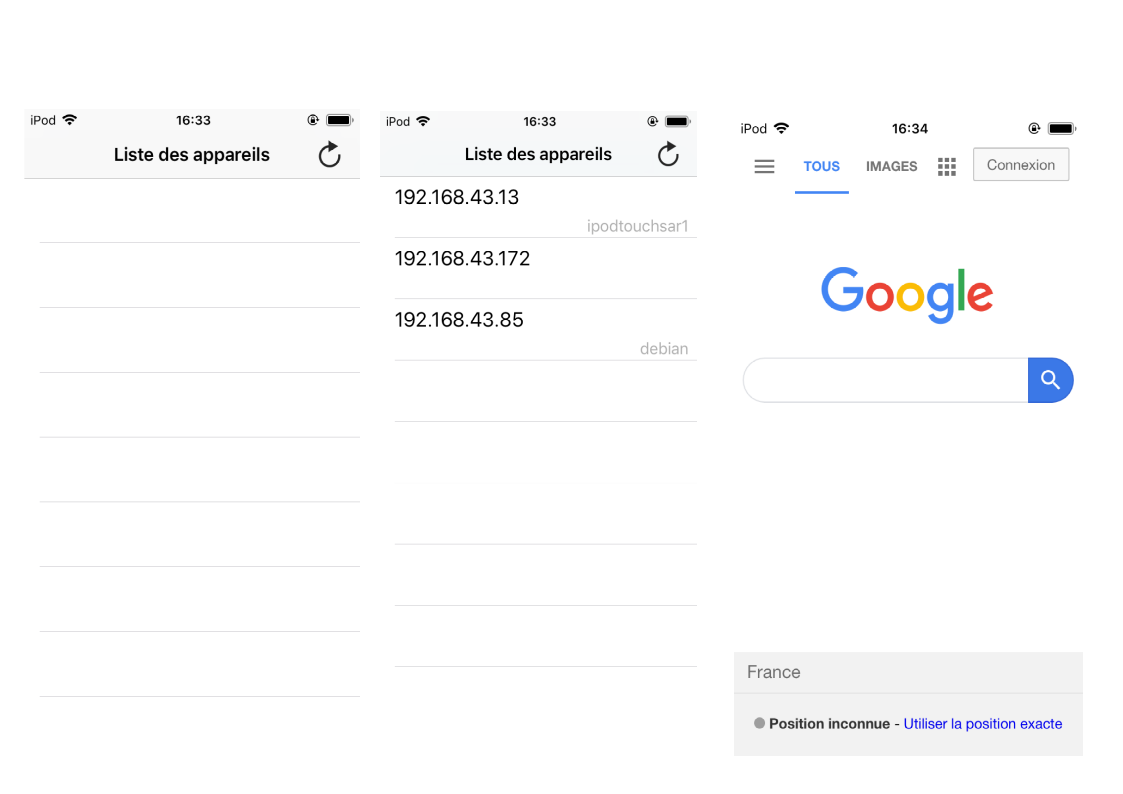
\includegraphics[scale=0.37]{ipod.png}
		\end{center}
	\end{frame}
	
		\begin{frame}
	\section{Interface Utilisateur}
		\begin{center}
		\frametitle{Interface Utilisateur}
		%\subsection{Contraintes}
        %\framesubtitle{Les solutions}
        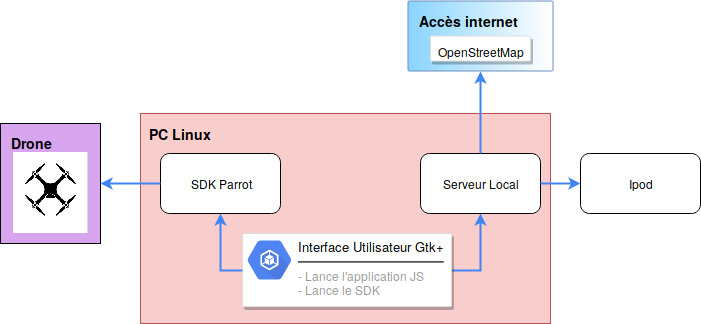
\includegraphics[scale=0.4]{Interface_utilisateur.jpg}
		\end{center}
	\end{frame}
	
	\begin{frame}
	\section{Tests}
		\begin{center}
		\frametitle{Tests effectués}
		%\subsection{Contraintes}
        %\framesubtitle{Les solutions}
           	\begin{itemize}
                \item Connection au drone
                \item Envoi d'un fichier Mavlink
                \item Execution du plan de vol selon un fichier mavlink enregistré sur le drone
                \item Retour video avec l'application ios à partir d'une url sur un serveur Linux
            \end{itemize}
		\end{center}
	\end{frame}
	
		\begin{frame}
		\begin{center}
		\frametitle{Problèmes rencontrés}
             \begin{itemize}
                \item Calibration du drone après chaque trajet effectué
                \item direction du drone durant le trajet
            \end{itemize}
		\end{center}
	\end{frame}
	
\end{document}


